\section{Introducción}
Ejemplo enumeración:
\begin{enumerate}
	\item Item1
	\item Item2
\end{enumerate}
Aquí se referencia a la imagen \ref{prueba} y aquí a la imagen \ref{prueba_invertida}

Ejemplo figura:
\begin{figure}[h]
	\centering
	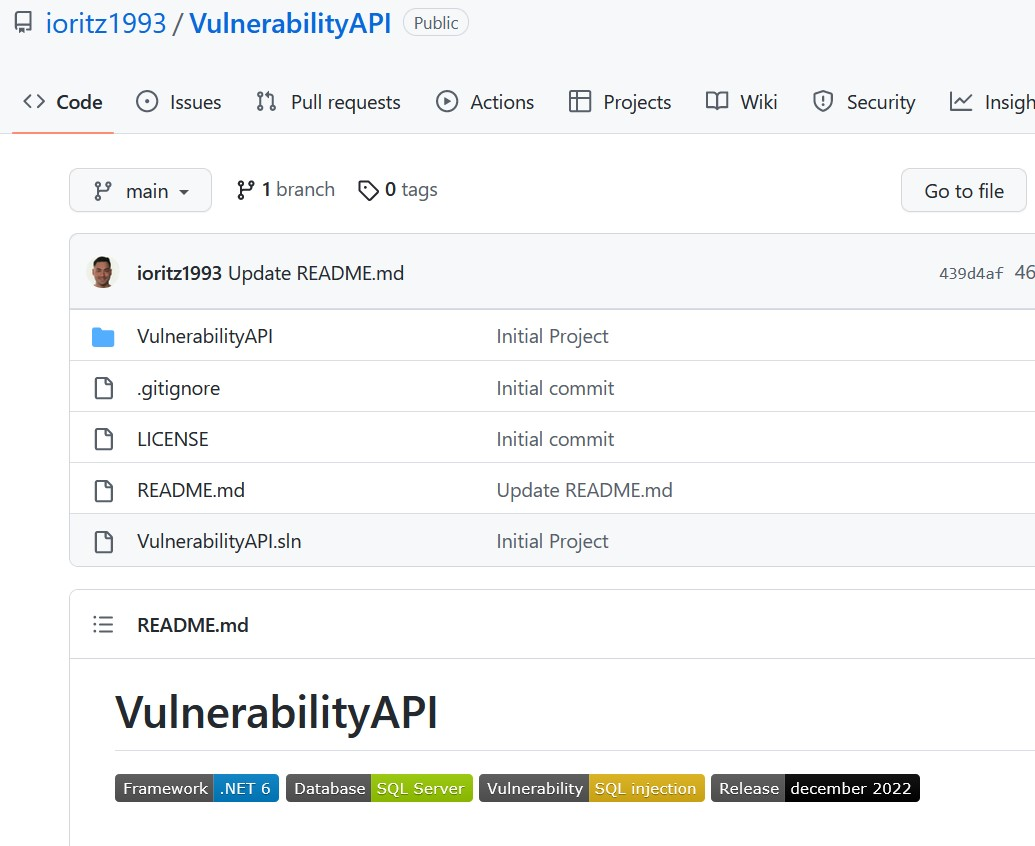
\includegraphics[width=160mm]{includes/ejemplo_figura.jpg}
	\caption[Ejemplo figura]{Ejemplo figura (Elaboración propia)}
	\label{prueba}
\end{figure} 

\begin{figure}[h]
	\centering
	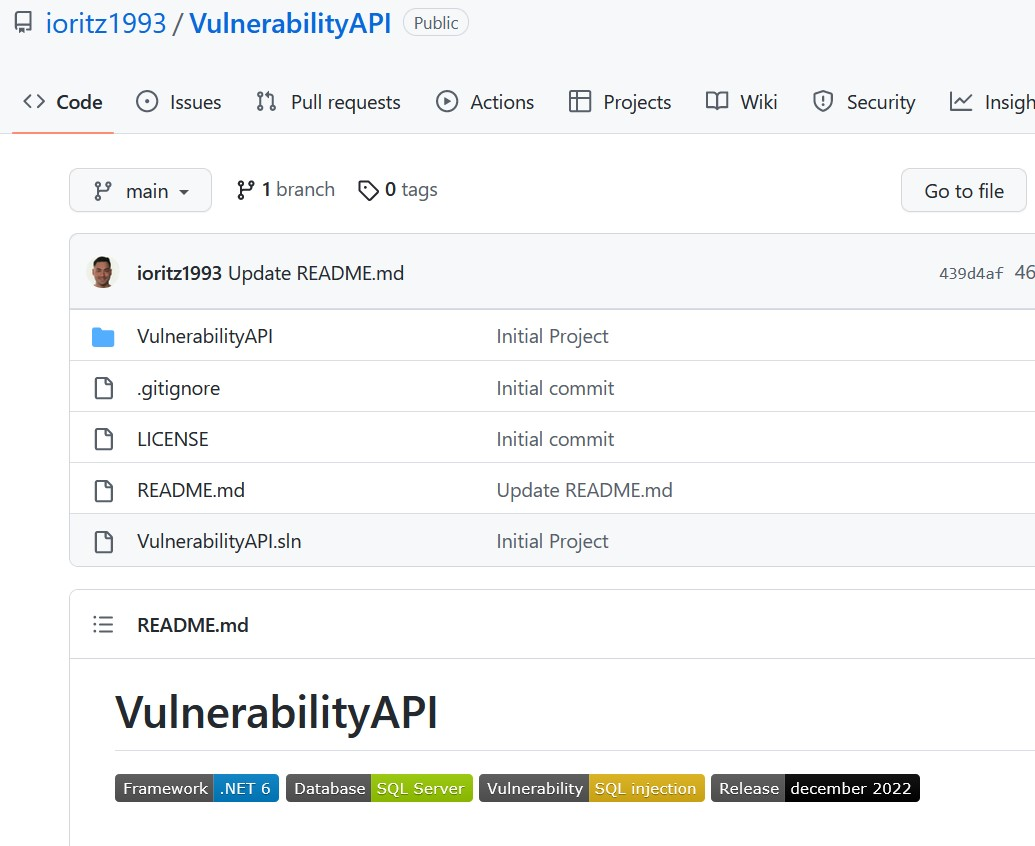
\includegraphics[width=160mm, angle=180]{includes/ejemplo_figura.jpg}
	\caption[Ejemplo figura girada]{Ejemplo figura girada (Elaboración propia)}
	\label{prueba_invertida}
\end{figure} 

